% System architecture of protocol v2 (single column).
\documentclass[tikz,border=2pt]{standalone}
\usepackage{newtxtext,newtxmath}
\usetikzlibrary{arrows.meta,fit,backgrounds}
\begin{document}
\footnotesize
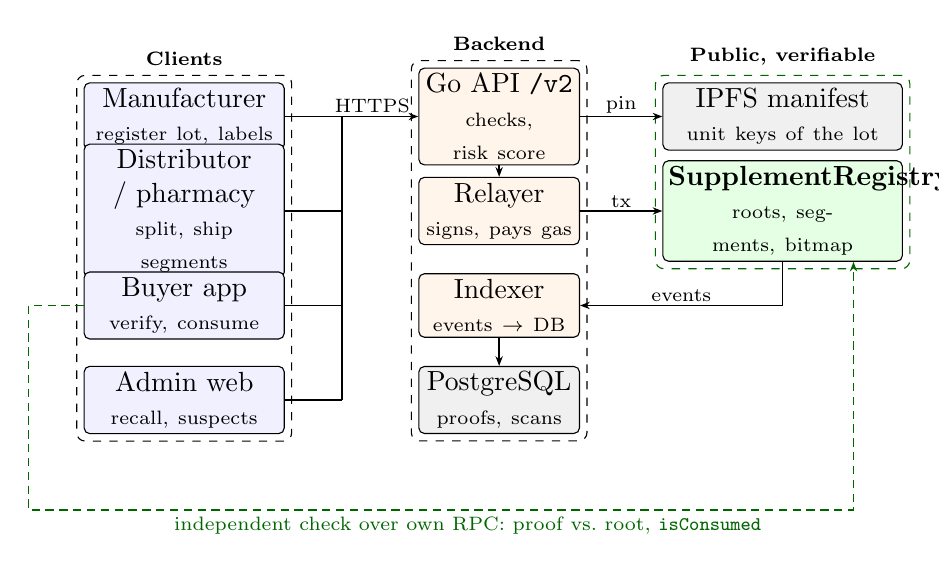
\begin{tikzpicture}[
  x=1mm, y=1mm,
  >={Stealth[length=3.5pt]},
  box/.style={draw, rounded corners=2pt, align=center, inner sep=2pt, minimum height=8mm, fill=white},
  app/.style={box, fill=blue!6, text width=24mm},
  svc/.style={box, fill=orange!8, text width=19mm},
  chain/.style={box, fill=green!10, text width=29mm, minimum height=10mm},
  store/.style={box, fill=gray!12},
  group/.style={draw, dashed, rounded corners=3pt, inner sep=2.5pt},
  lbl/.style={font=\scriptsize, inner sep=1pt},
  flow/.style={->, semithick},
  check/.style={->, semithick, densely dashed, green!40!black},
  small/.style={font=\scriptsize},
]
  \node[app] (mfr)   at (0,0)   {Manufacturer\\{\scriptsize register lot, labels}};
  \node[app] (dist)  at (0,-12) {Distributor / pharmacy\\{\scriptsize split, ship segments}};
  \node[app] (buyer) at (0,-24) {Buyer app\\{\scriptsize verify, consume}};
  \node[app] (admin) at (0,-36) {Admin web\\{\scriptsize recall, suspects}};

  \node[svc] (api)   at (40,0)   {Go API \texttt{/v2}\\{\scriptsize checks, risk score}};
  \node[svc] (relay) at (40,-12) {Relayer\\{\scriptsize signs, pays gas}};
  \node[svc] (idx)   at (40,-24) {Indexer\\{\scriptsize events $\to$ DB}};
  \node[store, text width=19mm] (pg) at (40,-36) {PostgreSQL\\{\scriptsize proofs, scans}};

  \node[store, text width=29mm] (ipfs) at (76,0) {IPFS manifest\\{\scriptsize unit keys of the lot}};
  \node[chain] (reg) at (76,-12) {\textbf{SupplementRegistryV2}\\{\scriptsize roots, segments, bitmap}};

  \begin{scope}[on background layer]
    \node[group, fit=(mfr)(admin), label={[small, font=\scriptsize\bfseries]above:Clients}] {};
    \node[group, fit=(api)(pg), label={[small, font=\scriptsize\bfseries]above:Backend}] {};
    \node[group, draw=green!40!black, fit=(ipfs)(reg), label={[small, font=\scriptsize\bfseries]above:Public, verifiable}] {};
  \end{scope}

  % every client talks HTTPS to the API
  \foreach \c in {mfr, dist, buyer, admin} \draw[semithick] (\c.east) -- (20,0 |- \c.east);
  \draw[semithick] (20,0 |- mfr.east) -- (20,0 |- admin.east);
  \draw[flow] (20,0) -- node[lbl, above, pos=0.4] {HTTPS} (api.west);

  \draw[flow] (api) -- (relay);
  \draw[flow] (api.east) -- node[lbl, above] {pin} (ipfs.west);
  \draw[flow] (relay.east) -- node[lbl, above] {tx} (reg.west);
  \draw[flow] (reg.south) |- node[lbl, above, pos=0.75] {events} (idx.east);
  \draw[flow] (idx) -- (pg);

  % the buyer's app re-checks the API's answer against the chain
  \draw[check] (buyer.west) -- ++(-7,0) |- (60,-50) -| ([xshift=9mm]reg.south);
  \node[lbl, text=green!40!black, anchor=north] at (36,-50.5) {independent check over own RPC: proof vs.\ root, \texttt{isConsumed}};
\end{tikzpicture}
\end{document}
